%%%%%%%%%%%%%%%%%%%%%%%%%%%%%%%%%%%%%%%%%%%%%%%%%%%%%%%%%%%%%%%%%%%%%%
% Source: Dave Richeson (divisbyzero.com), Dickinson College
% Version francaise par Vincent Pantaloni, prof.pantaloni.free.fr
% Traduction, correction et adaptation à la typographie française.
%
% Feel free to distribute this example, but please keep the referral
% to divisbyzero.com
% 
%%%%%%%%%%%%%%%%%%%%%%%%%%%%%%%%%%%%%%%%%%%%%%%%%%%%%%%%%%%%%%%%%%%%%%
%
%%%%%%%%%%%%%%%%%%%%%%%%%%%%%%%%%%%%%%%%%%%%%%%%%%%%%%%%%%%%%%%%%%%%%%

\documentclass[a4paper,10pt,landscape]{article}
\usepackage{fontspec}
\usepackage{amssymb,amsmath,amsthm,amsfonts}
\usepackage{multicol,multirow}
\usepackage{calc}
\usepackage{ifthen}
\usepackage{microtype}
\usepackage{url}



\usepackage[landscape]{geometry}
\usepackage[colorlinks=true,citecolor=blue,linkcolor=blue]{hyperref}
\usepackage{tikz}
\usepackage[most]{tcolorbox}
\usepackage{xcolor}

% Define custom colors
\definecolor{warningyellow}{RGB}{255,204,0}
\definecolor{warningred}{RGB}{204,0,0}

% Create a new tcolorbox style for warnings
\newtcolorbox{warningbox}[1][]{%
  enhanced,
  colback=warningyellow!10,
  colframe=warningred,
  boxrule=1pt,
  title=Warning,
  fonttitle=\bfseries,
  coltitle=white,
  top=2mm,
  bottom=2mm,
  left=2mm,
  right=2mm,
  arc=1mm,
  title style={top color=warningred,bottom color=warningred},
  #1
}
\usetikzlibrary{arrows.meta}

\ifthenelse{\lengthtest { \paperwidth = 11in}}
    { \geometry{top=.5in,left=.5in,right=.5in,bottom=.5in} }
	{\ifthenelse{ \lengthtest{ \paperwidth = 297mm}}
		{\geometry{top=1cm,left=1cm,right=1cm,bottom=1cm} }
		{\geometry{top=1cm,left=1cm,right=1cm,bottom=1cm} }
	}
\pagestyle{empty}
\makeatletter
\renewcommand{\section}{\@startsection{section}{1}{0mm}%
                                {-1ex plus -.5ex minus -.2ex}%
                                {0.5ex plus .2ex}%x
                                {\normalfont\large\bfseries}}
\renewcommand{\subsection}{\@startsection{subsection}{2}{0mm}%
                                {-1explus -.5ex minus -.2ex}%
                                {0.5ex plus .2ex}%
                                {\normalfont\normalsize\bfseries}}
\renewcommand{\subsubsection}{\@startsection{subsubsection}{3}{0mm}%
                                {-1ex plus -.5ex minus -.2ex}%
                                {1ex plus .2ex}%
                                {\normalfont\small\bfseries}}
\makeatother
\setcounter{secnumdepth}{0}
\setlength{\parindent}{0pt}
\setlength{\parskip}{0pt plus 0.5ex}


% -----------------------------------------------------------------------

\begin{document}

\raggedright
\footnotesize

\begin{center}
    {\Large\textbf{CS2109\textsubscript{s} Cheatsheet, by randomwish}}\\[0.5em]
    \url{https://github.com/randomwish/schoolNotes}
\end{center}
\begin{multicols}{3}
\setlength{\premulticols}{1pt}
\setlength{\postmulticols}{1pt}
\setlength{\multicolsep}{1pt}
\setlength{\columnsep}{2pt}

\section{"Traditional" AI}

\subsection{Definition of Intelligent Agents}
Consists of a \textbf{feedback loop} consisting of \textbf{sensors}, \textbf{functions}, \textbf{actuators} and
the actual \textbf{environment} (also known as \textbf{PEAS}).
\begin{itemize}
    \item \textbf{Performance measure} $\rightarrow$ used to consider metric to optimise for the right purpose
    \item \textbf{Rational agent} $\rightarrow$ chooses actions which would maximise performance measure
    \item \textbf{function} $\rightarrow$ maps from percept histories to actions: 
    $f : [\mathcal{P}^* \rightarrow \mathcal{A}$]
\end{itemize}


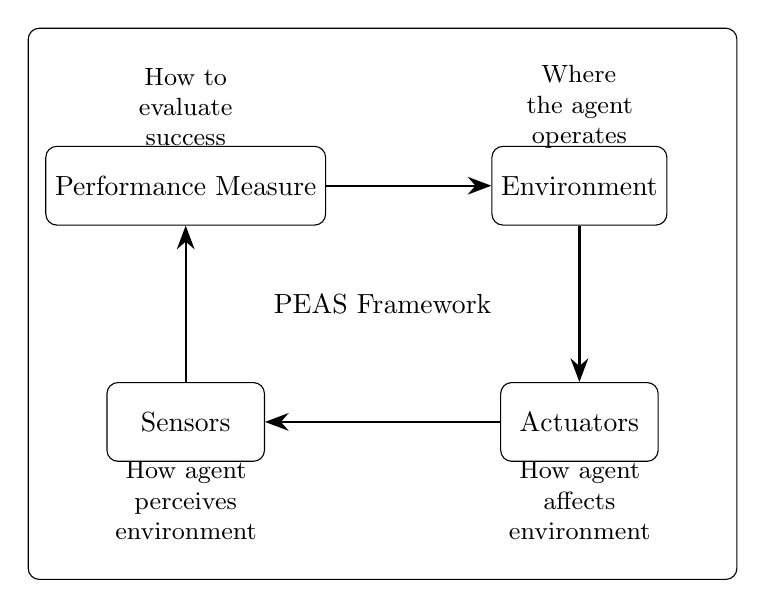
\begin{tikzpicture}[
    box/.style={draw, rectangle, minimum width=2cm, minimum height=1cm, text centered, rounded corners},
    arrow/.style={-{Stealth[length=3mm]}, thick}
]

% Main PEAS box
\node[box, minimum width=9cm, minimum height=7cm] (peas) at (0,0) {PEAS Framework};

% Individual components
\node[box] (p) at (-2.5,1.5) {Performance Measure};
\node[box] (e) at (2.5,1.5) {Environment};
\node[box] (a) at (2.5,-1.5) {Actuators};
\node[box] (s) at (-2.5,-1.5) {Sensors};

% Arrows connecting components
\draw[arrow] (p) -- (e);
\draw[arrow] (e) -- (a);
\draw[arrow] (a) -- (s);
\draw[arrow] (s) -- (p);

% Labels
\node[text width=2cm, align=center, font=\small] at (-2.5,2.5) {How to evaluate success};
\node[text width=2cm, align=center, font=\small] at (2.5,2.5) {Where the agent operates};
\node[text width=2cm, align=center, font=\small] at (2.5,-2.5) {How agent affects environment};
\node[text width=2cm, align=center, font=\small] at (-2.5,-2.5) {How agent perceives environment};

\end{tikzpicture}
\subsection{Categories of task environments}
\textbf{observability}
\begin{itemize} 
    \item fully observable $\rightarrow$ sensors of agents give it access to complete state of the environment at each point in time
    \item partially observable $\rightarrow$ sensors of agent do not have complete information
\end{itemize}

\textbf{deterministic}
\begin{itemize}
    \item deterministic $\rightarrow$ next state of environment is \textbf{completely} determined by current state and action executed by agent
    \item stochastic $\rightarrow$ state of environment is also determined by \textbf{chance} or \textbf{randomness}
    \item strategic $\rightarrow$ deterministic environment except for the actions of other agents
\end{itemize}

\textbf{types of experience for an agent}
\begin{itemize}
    \item episodic environment $\rightarrow$ experience of agent is divided into atomic episodes, and choice of agent depends \textbf{only} on the episode
    \item sequential environment $\rightarrow$ experience of agent makes it such that the choice of agent happened in the past
\end{itemize}

\textbf{whether environment changes}
\begin{itemize}
    \item static $\rightarrow$ environment does not change over time
    \item semi-dynamic $\rightarrow$ environment does not change with time, but agent's performance does
    \item dynamic $\rightarrow$ environment changes over time
\end{itemize}

\textbf{number of possibilities}
\begin{itemize}
    \item discrete $\rightarrow$ a limited number of distinct, clearly defined percepts and actions
    \item continuous $\rightarrow$ \textit{continuous} number of positions for an agent to be in
\end{itemize}

\textbf{number of agents}
\begin{itemize}
\item single agent $\rightarrow$ an agent operating by itself
\item multi-agent $\rightarrow$ a group of agents operating
\end{itemize}


\subsection{Types of agents}
\subsubsection{Simple reflex agent}
Only consists of a condition-action rule; akin to a if-else sequence
\subsubsection{Model-based agent}
agent is able to know its future effect of its actions; has a model of the environment
\subsubsection{Goal-based agent}
agent is able to \textbf{simulate} its future actions to reach its intended goal
\subsubsection{Utility-based agent}
define the utility/value in being at a given state of the environment
\subsubsection{Learning agent}
agent interact with environment and from interactions, produce trajectories with a learning model (learnt intuition)

\begin{warningbox}
All agents have PEAS, regardless of their types
\end{warningbox}
\subsection{Exploration vs Exploitation}
\begin{itemize}
    \item exploration $\rightarrow$ to learn more about the world
    \begin{itemize}
    \item downside $\rightarrow$ could lead to worse outcomes 
    \end{itemize}
    \item exploitation $\rightarrow$ maximise gain based on current knowledge
    \begin{itemize}
    \item downside $\rightarrow$ might not lead to better outcomes
    \end{itemize}
\end{itemize}
\end{multicols}

\end{document}
